%!TEX root = ../thesis.tex
\renewcommand{\Q}{\scr Q}


We will assume the entire graph has no separating 3 or 4 cycles. We will show that in this case ...

\section{Some Definitions}
  \subsubsection{More chords}
    Recall that a \emph{chord} of a path $\P$ is a edge that connects two non-subsequent vertices of that path. Note that this edge can't be in the path. A \emph{k-chord} is a path $\Q$ of $k$ edges that connects two nonsubsequent vertices $v_i, v_j$ of the path such that $\P \cap \Q = \braces{v_i, v_j}$.

    Note that $\P|_{v_i, v_j} \oplus \rev(\Q)$ is a cycle. We call this chord \emph{separating} if this is a separating cycle. \fxnote{Define Rev}


  \subsubsection{The neighbor walk of a path}
    \fxwarning{Note that the same/similar things hold for the left boundary walk}
    During this proof we will frequently use the concept of the right neighbor walk of a path.
    Given a path $P = p_1 \ldots p_k$ in a graph $G$
    The \emph{right neighbor walk} $W$ of $P$ will consist of $p_1$ and the vertices adjacent to $p_{2}$ between $p_1$ and $p_{3}$ in the clockwise rotation at $p_{2}$ followed by the vertices between $p_{2}$ and $p_{4}$ in the rotation at $p_{3}$ and so further until we add the vertices between $p_{k-2}$ and $p_k$ in the rotation around $p_{k-1}$ and finally we finish by adding $p_k$ to $W$.
    We then remove all subsequent duplicates from $W$

    \begin{lemma}
      \label{lm:uni:neighborWalk}
      The right neighbor walk $W$ is a walk.
    \end{lemma}
    \begin{proof}
      Let $w$ and $w'$ be two subsequent vertices in $W$. We will show they are connected. We first consider the case $\braces{w, w'} \cap \braces{p_1, p_k } = \emptyset$.
      Now there are two cases. Either $(a)$ $w$ and $w'$ are vertices adjacent to some $p_i$ an thus subsequent in the rotation at $p_i$  or $(b)$ $w$ was the last vertex adjacent to some $p_i$ and thus $w'$ is the first vertex adjacent to $p_{i+1}$.

      The following two situations can also be seen in Figure \ref{fig:uni:walkproof}.

      \begin{figure}[h]
          \centering
          \begin{subfigure}[b]{0.5\linewidth}
              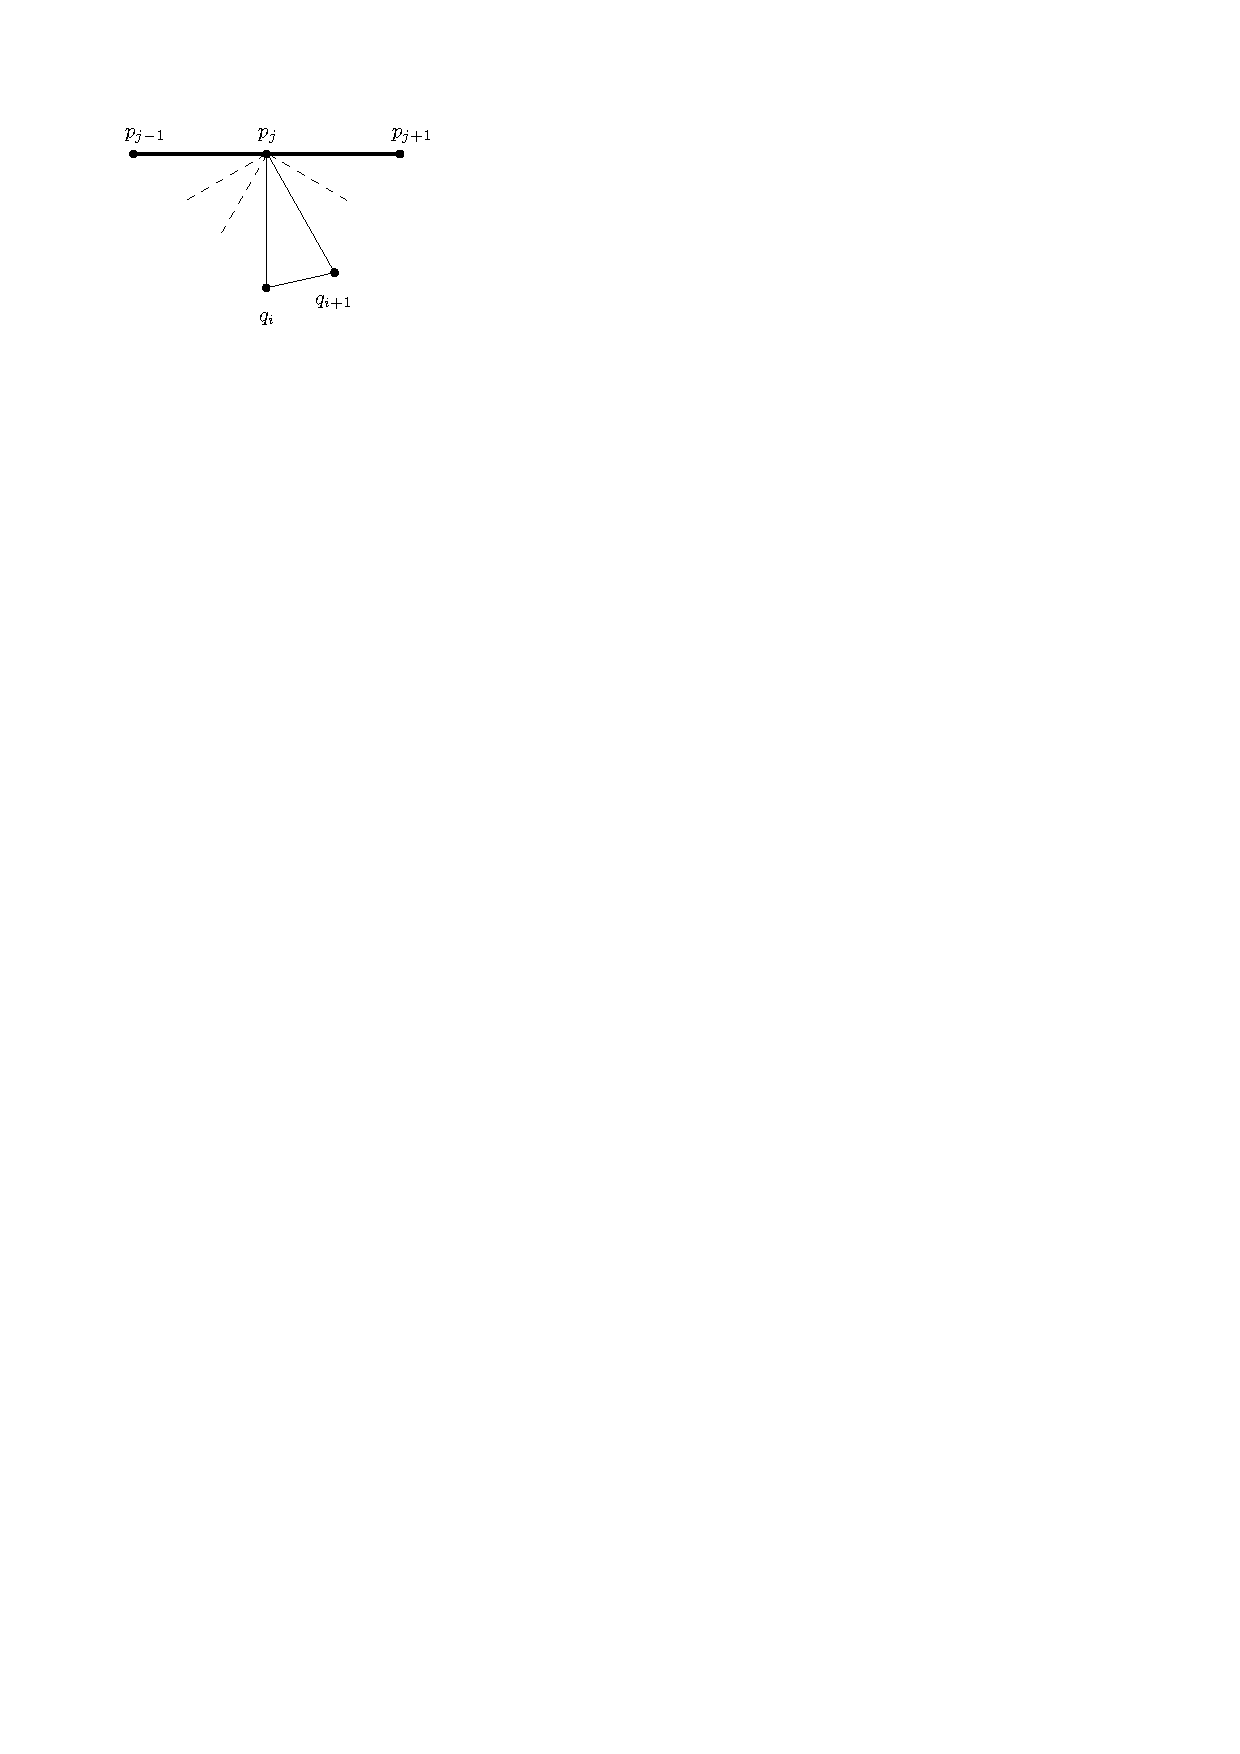
\includegraphics[width=\linewidth]{unifiedAlgo/img/walkProofA}
              \caption{}
          \end{subfigure}%
          \begin{subfigure}[b]{0.5\linewidth}
              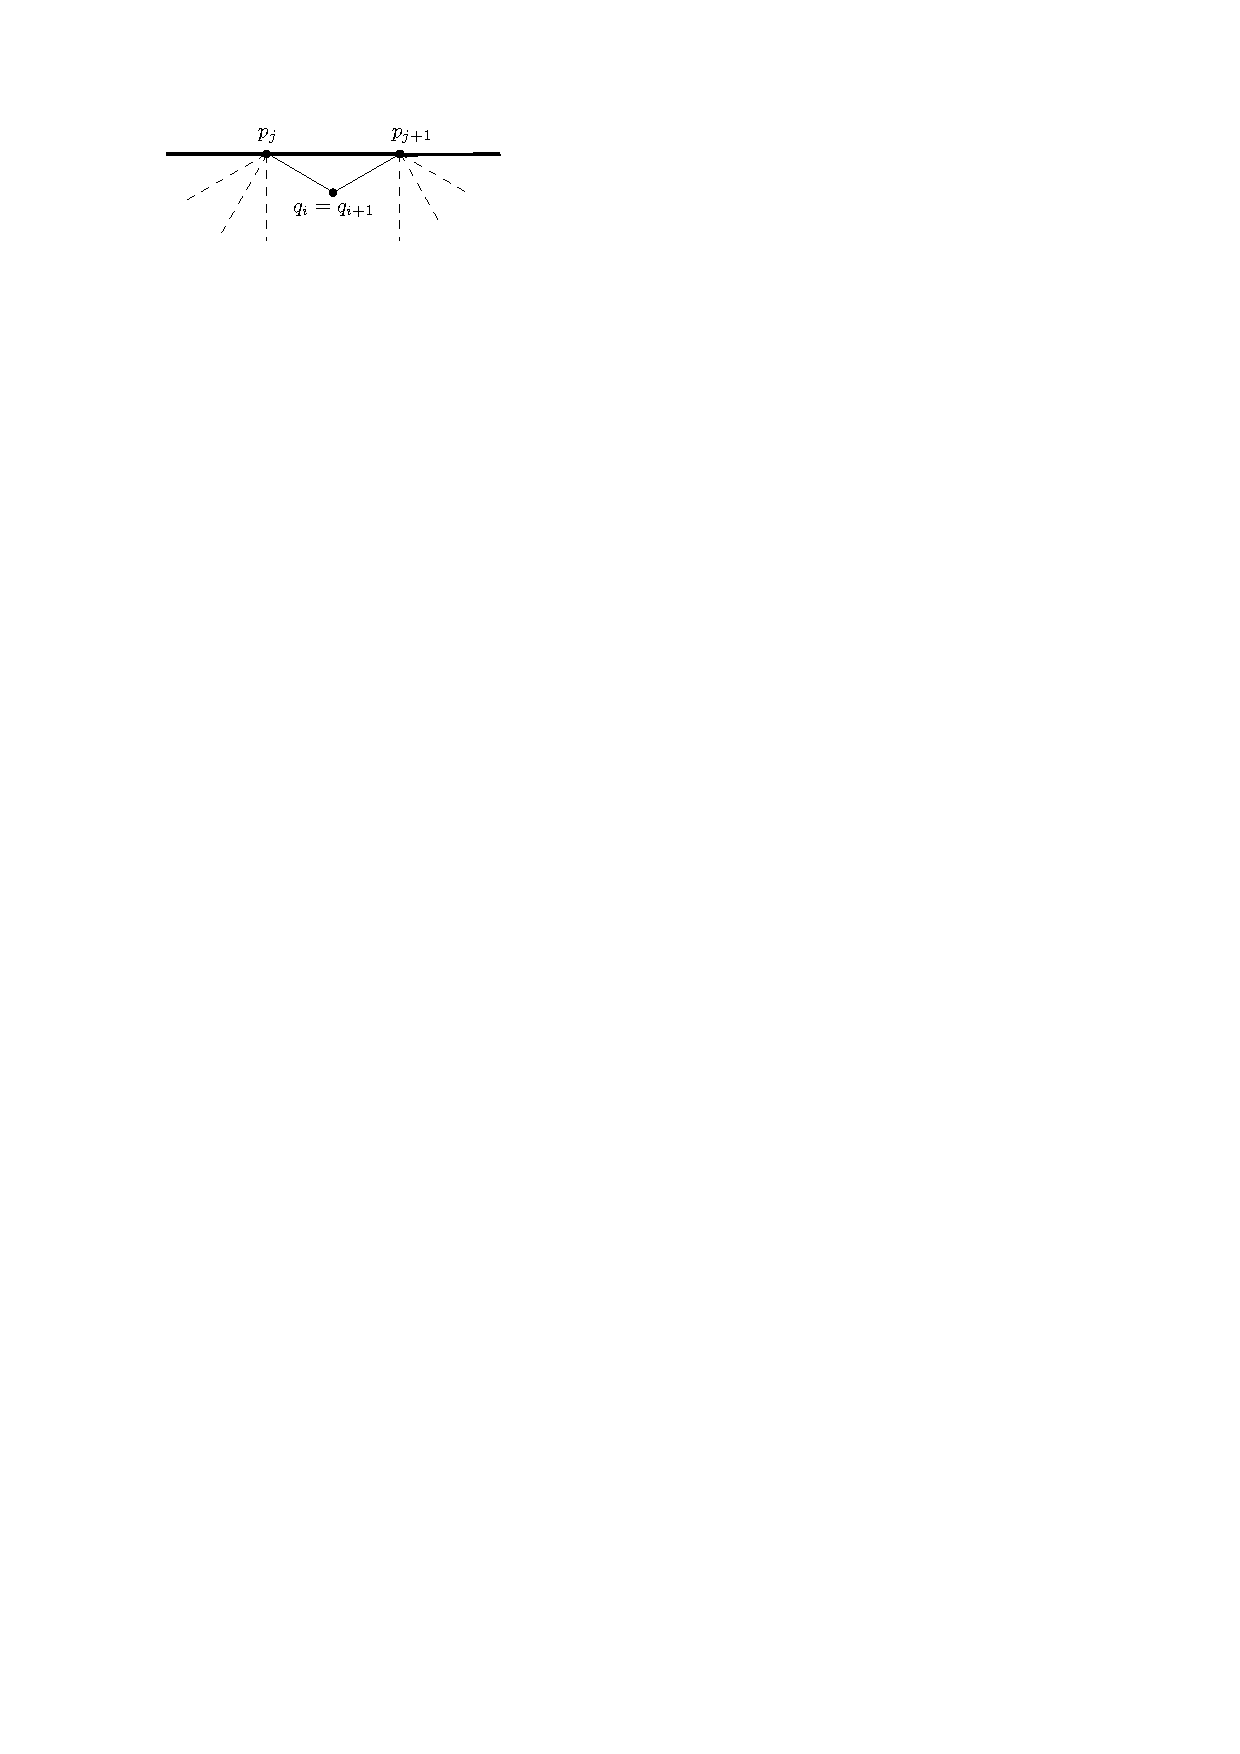
\includegraphics[width=\linewidth]{unifiedAlgo/img/walkProofB}
              \vspace{1cm}

              \caption{}
          \end{subfigure}

            \caption{The two main cases of the proof showing that $W$ is a walk}
        \label{fig:uni:walkproof}
      \end{figure}

      In case $(a)$ we note that since $w$ and $w'$ are subsequent in the rotation at $p_i$ $ww'$ is an edge by Lemma \ref{lm:prelim:rotationEdge}.

      In case $(b)$ we note that $p_i w$ and $p_i p_{i+1}$ are edges subsequent in clockwise order, hence $wp_{i+1}$ is also an edge. Hence $w$ is the first vertex adjacent to $p_{i+1}$ subsequent to $v_i$ in the clockwise rotation. Thus $w= w'$. They are duplicates and one of them must have been removed.

      Now for the edge cases: Let $x$ be the first vertex adjacent to $p_{i+1}$ and let $y$ be the last vertex adjacent to $p_{j-1}$. $p_i$ and $x$ are vertices adjacent to $p_{i+1}$ subsequent in the clockwise rotation, and hence connected by Lemma \ref{lm:prelim:rotationEdge}. In the same way $y$ and $v_j$ are subsequent vertices in the rotation at $v_n$ and hence connected.

      Hence $\W$ is a walk.
    \end{proof}


     \fxwarning{TODO Change to path iff I4 is satisfied}
    \begin{lemma}
      \label{lm:uni:neighborWalkNoncrossing}
      The right neighbor walk $W$ is a non-crosssing walk.
    \end{lemma}
    \begin{proof}
      Suppose that the right neighbor walk is crossing at a vertex $w= w_i =w_j$. Then one of $w_{j-1}$ and $w_{j+1}$ is in the clockwise interval $[w_{i-1}, w_{i+1} ]$ at the rotation at $w$. We will denote this vertex by $w'$. It is clear that $w'$ cannot be on the path unless $w'$ is $p_1$ or $p_k$. In this case however we see that $w_{i-1}$ or $w_{i+1}$ respectively couldn't have been part of the path.

      So we continue with $w'$ not on the path. All neighbors of $w$ between $w_{i-1}$ and $w_{i+1}$ in the clockwise rotation are on the path. \fxwarning{TODO make this a lemma}. So we have a series of triangles by Lemma \ref{lm:prelim:rotationEdge}. Now $w'$ must be inside one of these triangles, otherwise we would have a crossing edge (and thus a non-planar graph.) Now the triangle containing $w$ is a separating triangle.

      We conclude that $W$ must be a non-crossing walk.
    \end{proof}


    \fxnote{Actullly W rev(P)}
    \fxnote{Change wording to cycle}
    \begin{lemma}
      \label{lm:uni:neighbourwalkNoInteriorVertex}
      The closed non-crosing walk $WP$ has no interior vertex.
    \end{lemma}
    \begin{proof}subsequent
      The interior of $WP$ consists of only triangles with all vertices in $WP$. We can see this from the construction of the neighbor walk. Both cases in Figure \ref{fig:uni:walkproof} add a triangle to the interior with all vertices in $WP$.

      Suppose there is a interior vertex. Then the triangle containing this vertex is a separating triangle.
    \end{proof}


    \begin{lemma}
      \label{lm:uni:neighbourwalkChordFree}
      The left of the of a right neighbor walk is chordfree.
    \end{lemma}
    \begin{proof}
      Suppose that the right neighbor walk $W = w_1 \ldots w_k$  has a chord on the left, say between $w_i$ and $w_j$ with $i< j -1 $. There is a vertex $p_\ell \in P$ on the path such that $w_{i+1}$ is a neighbor of $p_\ell$ to the left of $p_\ell$ Consider now the following non-crossing closed walk $P w_k \ldots w_{j+1} w_j w_i w_{i-1} \ldots w_1$
      (Thick in Figure \ref{fig:uni:neihbourwalkChordFree})this walk has $w_{i+1}$ in its exterior. But then $p_\ell w_{i+1}$ is a crossing edge. Which is forbidden.

      \begin{figure}[h]
        \centering
        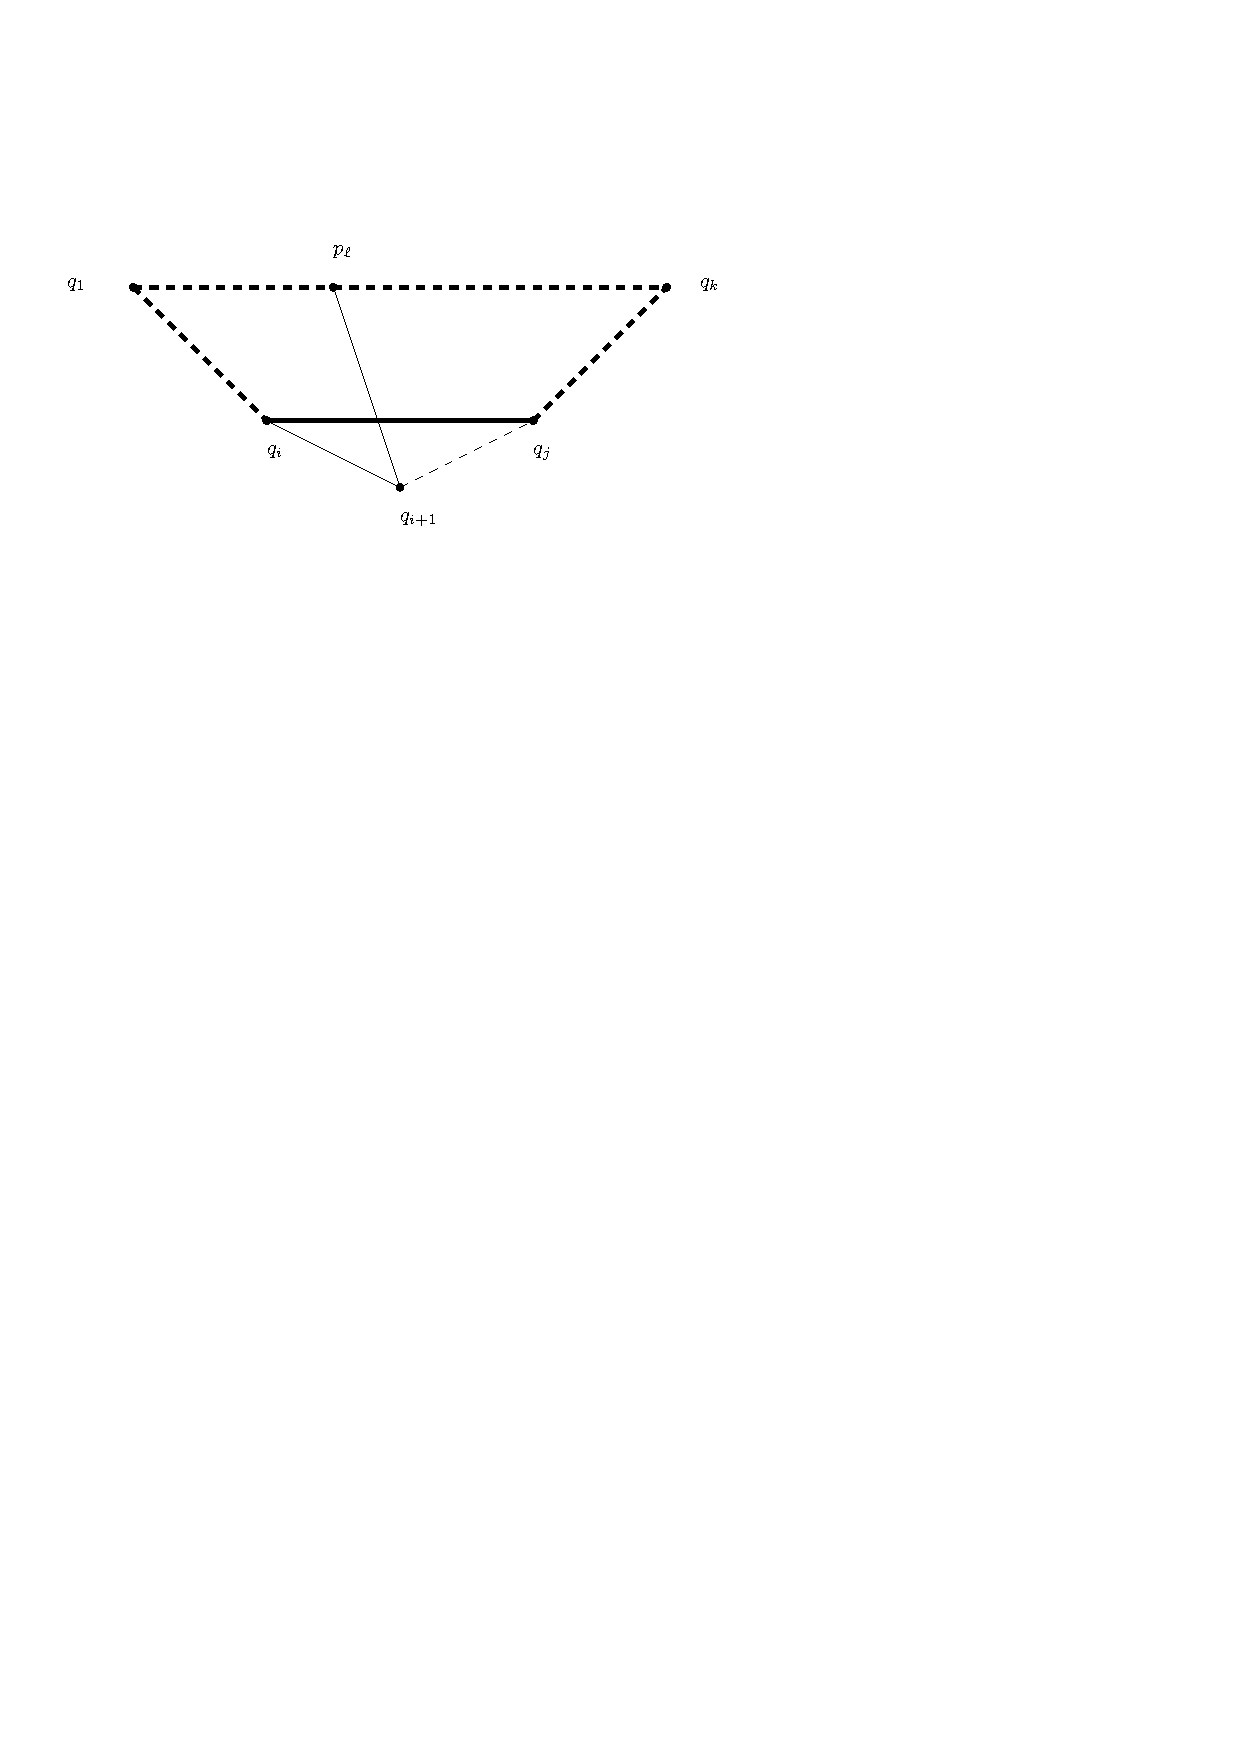
\includegraphics[scale=1]{unifiedAlgo/img/neighbourWalkChords}
        \caption{The construction in the proof of Lemma \ref{lm:uni:neighbourwalkChordFree}}
        \label{fig:uni:neihbourwalkChordFree}
      \end{figure}
    \end{proof}

    \fxnote{Alternate proof based on   ($\W$ being oriented from $\pW$ to $\pE$), since if it would lie on the left of $\W$ the vertices $w_{i+1},\ldots, w_{j-1}$ would not have been chosen in the construction of the prefence.}

\section{Algorithm}
  The algorithm will consist of two phases

  \begin{enumerate}
    \item Find a \emph{vertically} 1-sided layout with additional properties
    \item Do additional post-processing steps to make this layout $k$-sided.
  \end{enumerate}

\subsection{Phase 1}
  In Phase 1 we execute a sweepcycle algorithm comparable to Fusy's \cite{Fusy2006}.
  During the algorithm we will want to maintain several invariants. The first three are equivalent to those imposed by Fusy. The final two invariants are new and impose a nice structure on the sweepcycle so far.

  \begin{invariants}
    \itemsep=-4pt

    \item \label{i:uni:SWandSE} The cycle $\C$ contains the two edges $\pS \pW$ and $\pS \pE$.
    \item \label{i:uni:noChords} $\cpath$ has no chords
    \item \label{i:uni:intVertCond} All inner edges of $T$ outside of $\C$ are colored and oriented in such that the inner vertex condition holds. %TODO what is the inner vertex condition
    \fxerror{We need to add a partial inner vertex condition}
    \item \label{i:uni:no2Chords} $\C\sm{\pW, \pS, \pE}$ has no separating 2-chords
  \end{invariants}


  \begin{defi}[Prefence]
  A prefence $\W$ is a interior path of $\C$ starting at $v_i \in \C$ and ending at $v_j \in \C$ a both adjacent to $\pS$
  \begin{enumerate}
    \itemsep=-4pt
    \renewcommand*{\labelenumi}{(P\arabic{enumi})}%
    \renewcommand*{\theenumi}{(P\arabic{enumi})}%

    \item  $\C_\W$ Has no interior vertex
    \label{p:noInteriorVertex}
    \item  $\W$ has no chords on the left     \label{p:Wchordfree}
    \item  $\restC{\W}$ has no chords on the right     \label{p:Cchordfree}
  \end{enumerate}
  \end{defi}

  We do the following
  \begin{enumerate}
    \itemsep=-4pt
    \item Find the right neighbor walk
    \item Evade any future irregularities
    \item Update with this valid path
  \end{enumerate}

  We then repeat this until the sweepcycle does not contain any more interior vertices.

  \paragraph{Find the right neighbor path}
    Let $v_i$ denote all the vertices of $\cpath$ in the following order $\pW =  v_1 \  v_2 \  \ldots v_{n-1} \  v_n = \pE$.
    Some intervals of these vertices will be adjacent to $\pS$. However, they can't be all adjacent to $S$ since then the sweepcycle would be non-separating since we assumed $G$ has no separating triangles. We denote by $v_i$ the last vertex of fist interval of vertices adjacent to $S$ and by $v_j$ the first vertex of the second interval.
    As candidate walk we will take the right neighbor path of $\braces{v_i, \ldots, v_j}$.

    \begin{lemma}
      \label{lm:uni:isPrefence}
    The collection $W$ described above is a prefence.
    \end{lemma}
    \begin{proof}
    $W$ is a walk by lemma \ref{lm:uni:neighborWalk}. Furthermore it is a path since any non-simple point would offend Invariant \ref{i:uni:no2Chords} of the sweepcycle.


    We note \ref{p:noInteriorVertex} holds due to Lemma \ref{lm:uni:neighbourwalkNoInteriorVertex}

    We note \ref{p:Wchordfree} holds due to Lemma \ref{lm:uni:neighbourwalkChordFree}.

    We note \ref{p:Cchordfree} holds due to invariant \ref{i:uni:noChords}.
    \end{proof}

    We then orient $\W$ from $v_i$ (the vertex closest to $\pW$)to $v_j$ (the vertex closest to $\pE$) and denote it's vertices by $w_1 \ldots w_k$.


    \subsubsection{Irregularities}
      \fxerror{Account for polebound 2-chords}
      Now the prefence we found can have several structures we want to avoid
      namely
      \begin{enumerate}
        \itemsep=-4pt
        \item Chords
        \item Separating 2-chords
      \end{enumerate}

      All of these structures are on the right of the prefence since the prefence satisfies \ref{p:Wchordfree} (no chords on the left) and \ref{p:noInteriorVertex} (no separating 2-chords on the left).

      What we do depends on the first obstacle we encounter. The \emph{range} of an obstacle will be given by it's start and end vertex.

      \fxwarning{TODO Rewrite this to be clear}
      \paragraph{First obstacle is a chord}
      If our precycle has any chords we look identify the them by their start and end vertex. Of the chords with the lowest start index we will consider the one with the largest end index.

      Now we have a group of chords with start and end vertices. What we do now depends on whether a 2-chord shows up.

      \emph{No 2-chord}
      We look at the chord with the smallest range (i.e. highest start $i_0$ and lowest end $j_0$) then we will look at the biggest chords still starting at $i_0$ or ending at $j_0$. Say that this chord goes from $i_1$ to $j_1$ then we augment the sweepcycle with $i_1 +1$ to $j_1 -1$.

      \emph{A 2-chord}
      We find a piece to augment with in the same way  but we terminate it just before the first closing 2-chord.

      \paragraph{First obstacle is a 2-chord}
      If this 2-chord contains a chord, just apply the rules for chords as given above. Otherwise terminate the prefence just before the end of the 2-chord.

      \fxwarning{TODO Rewrite this to be clear}

      \begin{lemma}
        \label{lm:}
        We always augment with a valid path
      \end{lemma}
      \begin{proof}
        By construction
      \end{proof}

      \begin{lemma}
        \label{lm:}
        The resulting REL is vertically one-sided
      \end{lemma}
      \begin{proof}
        This is the same as saying that the resulting regular edge labeling has no blue Z's

        There are two ways a blue Z can form either we start at a vertex just before a merge or we terminate on a vertex just after a split.

        For start point the following holds. Either we start adjacent to $\pS$ or we start due to a chord.

        For end points the following holds either we end adjacent to $\pS$, or due to a chord or 2-chord.


        We will first show that we can't have a start just after a merge.
        If the merge is due to the vertex being adjacent to $\pS$ then the previous vertex is also adjacent to $\pS$ and we have nowhere to go. \fxnote{provide figure}

        Suppose now we ended due to a chord or a 2-chord. Then the only reason to start on this place is due to a chord.

        If we start or end at a vertex adjacent to $\pS$ the diagonal edge can't exist. Because there is not enough space for moves that could have generated this ... (I Think)

        \fxerror{Work this out, no energy now}


      \end{proof}

\subsection{Phase 2}
  We will then do the following post-processing steps:

  \begin{enumerate}
    \item Do flips isolating large botfans.
    \item treat long chains of Z's
    \item handle the blue faces that are still large
  \end{enumerate}

  Before we start with these preprocessing steps let us define the blue faces as they are now as \emph{strips} that in some cases still have to be subdivided.

  \subsubsection{Phase 2.1}
    In every face we look for large (4 or more edges) topfans.

    \begin{invariants}
      \label{inv:uni:load}
      \item The edges on a fence obey the following $2$ loaded edges are followed by at least $1$ unloaded edge
    \end{invariants}

    For every sequence of large topfans not separated by large botfans we flip the following:
    1. Left rim of the first fan.
    2. The left rim of every further odd fan.
    3. The right rim of the last fan.

    In particular: For a large topfan not neighbored by any other large topfans we recolor both rims.

    Note that we only flip rims of a $T_+$.

    We don't flip the first and last edge we would normally flip in a strip. If this edge does not separate the large topfan from at least three top edges we dont flip these edges.

    \begin{lemma}
      \label{lm:uni:removingLargeB-fans}
      We create blue $(5, \infty)$-faces containing all the large topfans while obeying Invariant \ref{inv:uni:load}.
    \end{lemma}
    \begin{proof}
      TODO \fxwarning{TODO But easy by the above construction}
    \end{proof}

  \subsubsection{Phase 2.2}
    While doing this in a strip that (partially) lies above another face we can then create a chain of $Z$'s. We have two kinds of these chains with the same orientation and opposite orientation.

    See figure \ref{fig:uni:chains}

    \begin{figure}
      \centering
      \begin{subfigure}[b]{0.45 \textwidth}
          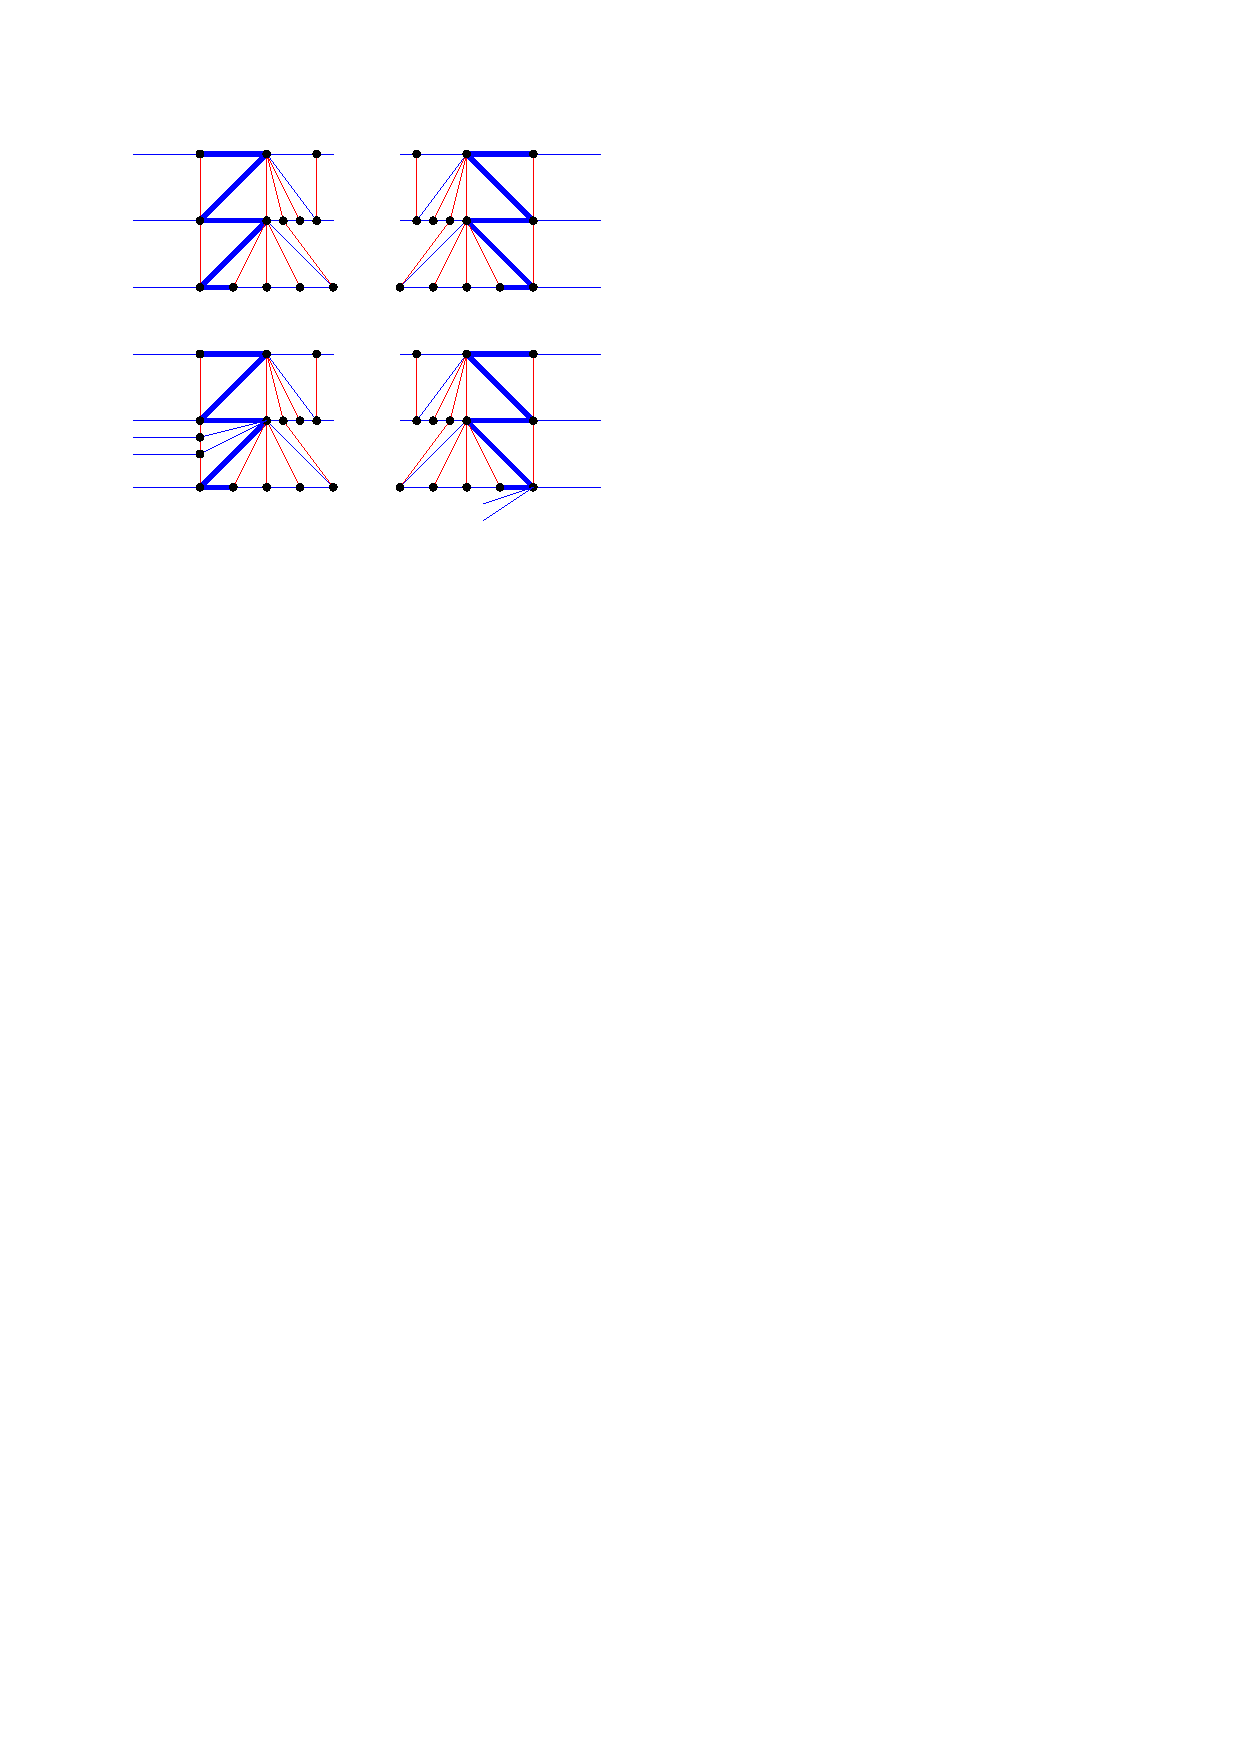
\includegraphics[width = \textwidth]{unifiedAlgo/img/post/sameChain}
          \caption{Same orientation}
      \end{subfigure}
      ~
      \begin{subfigure}[b]{0.45 \textwidth}
          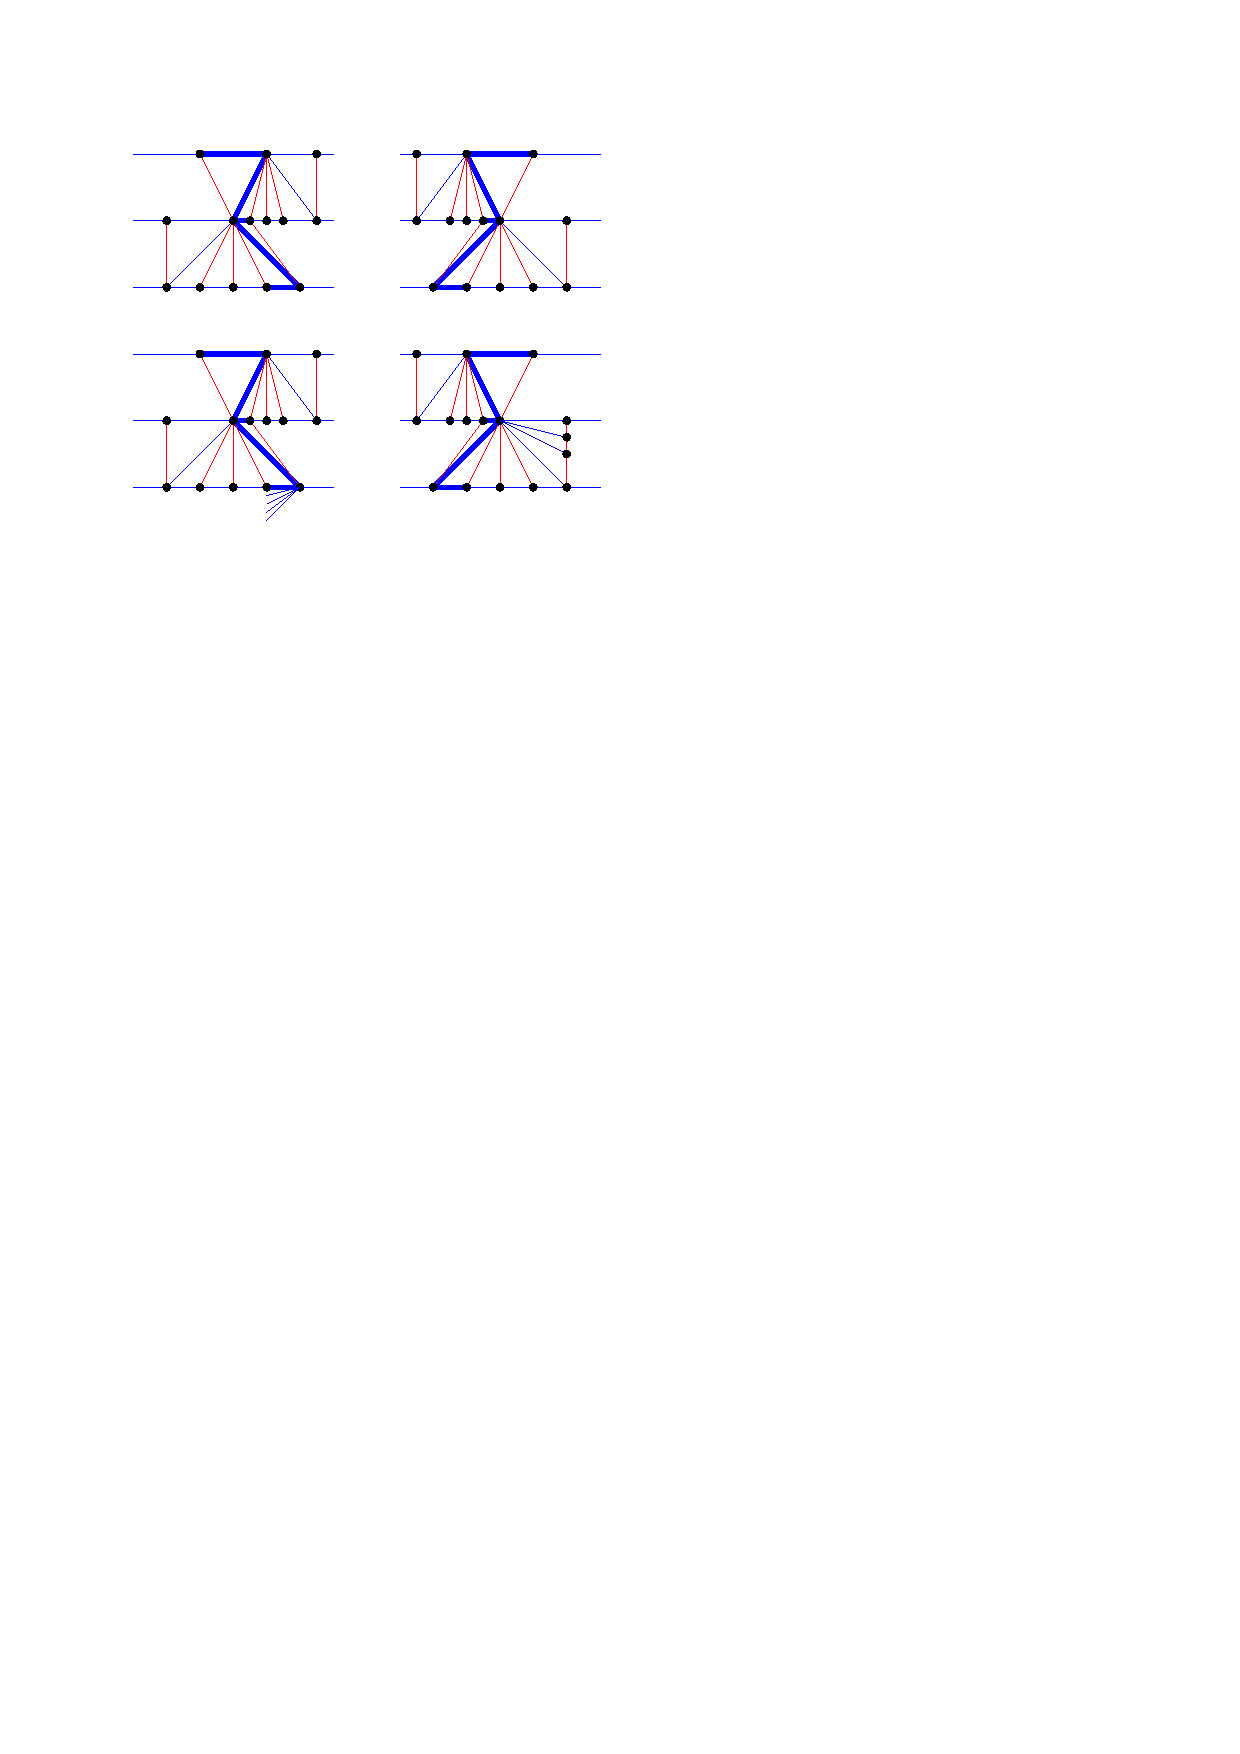
\includegraphics[width =\textwidth]{unifiedAlgo/img/post/oppChain}
          \caption{Opposite orientation}
      \end{subfigure}
      \caption{}
      \label{fig:uni:chains}
    \end{figure}

    From this phase we require the following.
    \begin{lemma}
      \label{lm:}
      After this phase all large topfans are in $9$-sided blue faces. All blue faces that are not $9$-sided consist of only $B$-fans and small $T$-fans.
    \end{lemma}

    \begin{proof}
      This follows from the way in which we entomb the large topfans.

      Clearly every large topfan is in a $9$-sided blue face. This even holds when we have a large topfan next to an opening and a closing of the face.
       \fxwarning{TODO small figure}

       By contraposition it is also clear that every face that is not $1$-sided cannot contain any large topfans and  thus consists of solely small topfans and botfans.
    \end{proof}

    We define a \emph{flip} as a series of changes to a REL turning it to another valid REL.
    We first do a flip turning every same orientation chain of $Z$'s to an opposite orientation one. Then we do a flip breaking an opposite orientation chain. We do this for every chain of $Z$'s created in Phase 2.1.

  We will work from the last created face upwards. When doing a flip we try to only alter the history, not the current face and certainly not the future. We will treat flips under a topfan of size 4 differently, because we don't have the space to execute all standard flips.

  \paragraph{Size of left joints}
  We will show the following

  \begin{defi}
    A \emph{left joint} is the vertex in a $Z$ with at least two outgoing blue edges.
  \end{defi}

  A left joint corresponds with a split.

  \begin{lemma}
    \label{lm:}
    A left joint not adjacent to $\pS$ with a split has no top fan below it.
  \end{lemma}
  \begin{proof}
    If we are not adjacent to $\pS$ the only reasons for a split vertex $v_i$ are a chord or a polebound separating 2-chord.

    We will first consider the case of a chord.

    Let $v_i$ denote the split vertex. And $v_j$ denote the vertex where the path that split off joined the sweepcycle again (merge vertex). The chord that causes (the bottommost represent of) this split and merge is from $w_i$ to $w_j$ with $v_i$ connected to $w_i$ and $w_{i+1}$ and $v_j$ to $w_j$ and $w_{j-1}$ (cf. chord and chord multi figures). (See description of evading a chord irregularity).

    Now in the next candidate walk $w_i$ and $w_j$ are next to each other and both have a $B$-fan of size at least $2$ (to $v_i$ and $w_{i+1}$ and to $v_j$ and $w_{j-1}$ respectively.)

  \end{proof}

  \paragraph{The standard flips}
  Figures of the basic same and opposite orientation flips.
   See Figure \ref{fig:uni:sameFlip}, \ref{fig:uni:sameFlipComplete} and \ref{fig:uni:oppFlip}.

  \paragraph{Flips under a topfan of size 4}
  Suppose we have a topfan $F$ of size $4$
  As long as there is only one chain of $Z$'s with one of the rims of $F$. We can just execute a regular flip without running out of space.




  \paragraph{Same orientation flip}

  In this case we do the flip in Figure \ref{fig:uni:sameFlip}

  \begin{figure}[h]
    \centering
    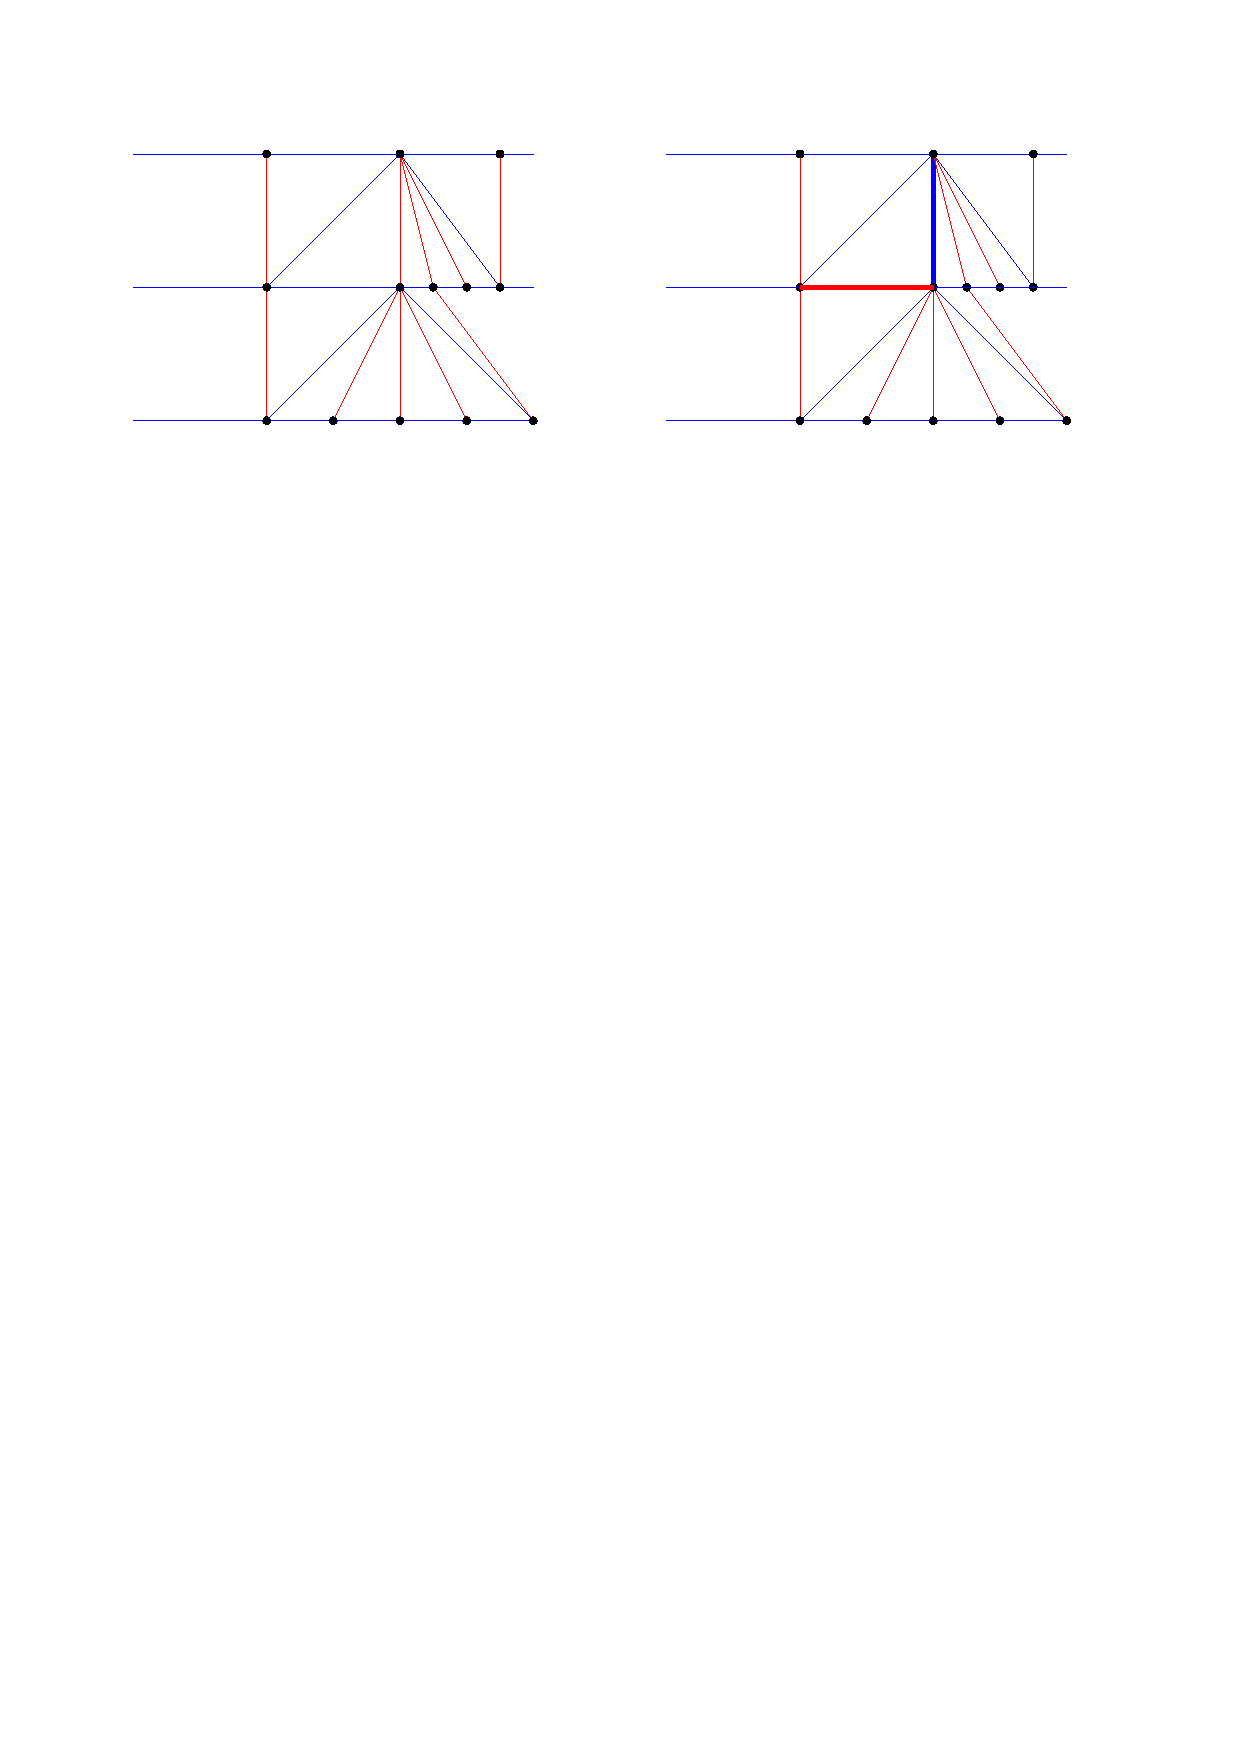
\includegraphics[width =\textwidth]{unifiedAlgo/img/post/sameFlip}
    \caption{The flip we execute on same direction chains}
    \label{fig:uni:sameFlip}
  \end{figure}

  \begin{figure}[h]
    \centering
    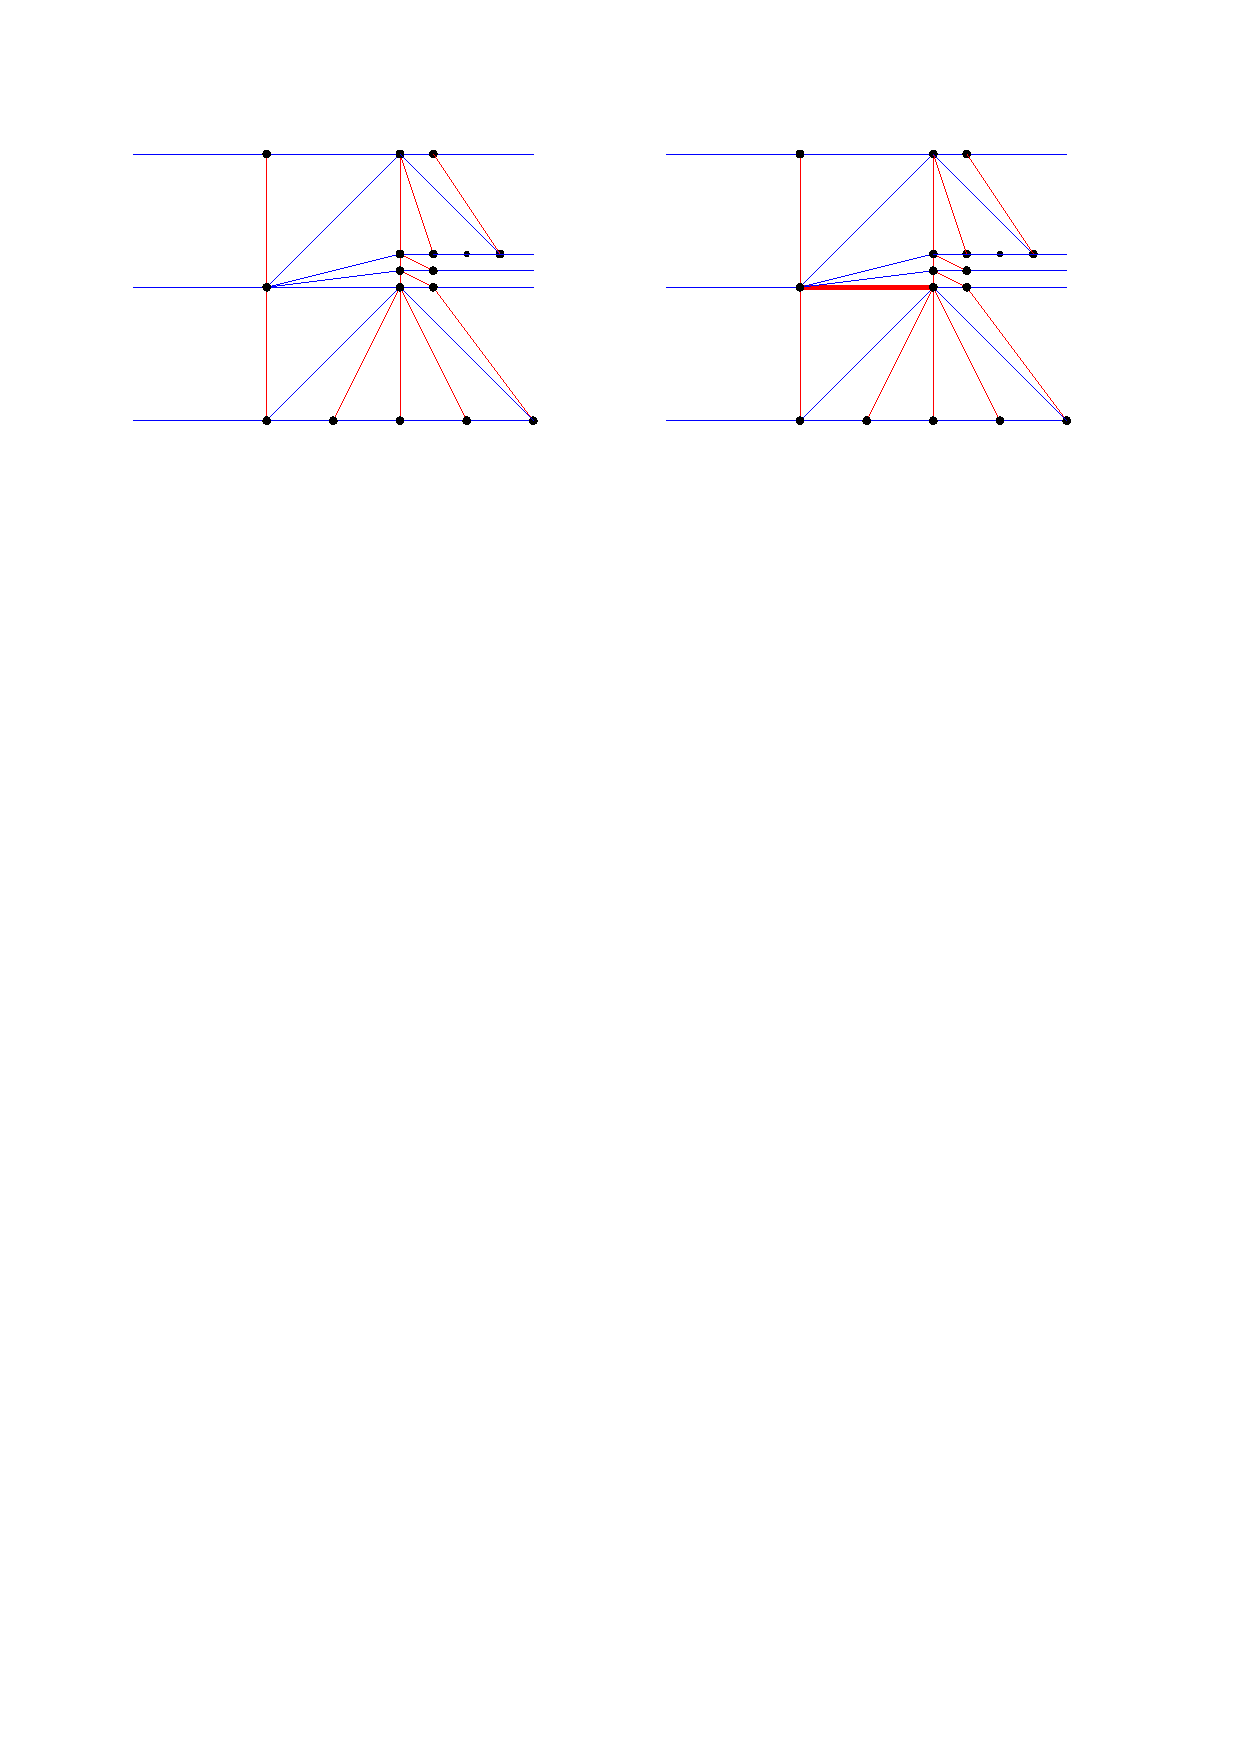
\includegraphics[width =\textwidth]{unifiedAlgo/img/post/sameMultiFlip}
    \caption{The flip we execute on same direction chains with multiple edges in the middle joint}
    \label{fig:uni:sameMultiFlip}
  \end{figure}

   after this flip we changed the chain and now we have a chain of oppositely oriented $Z$'s. Luckily we know how to treat these. See Figure \ref{fig:uni:sameFlipComplete}.

   \begin{figure}[h]
     \centering
     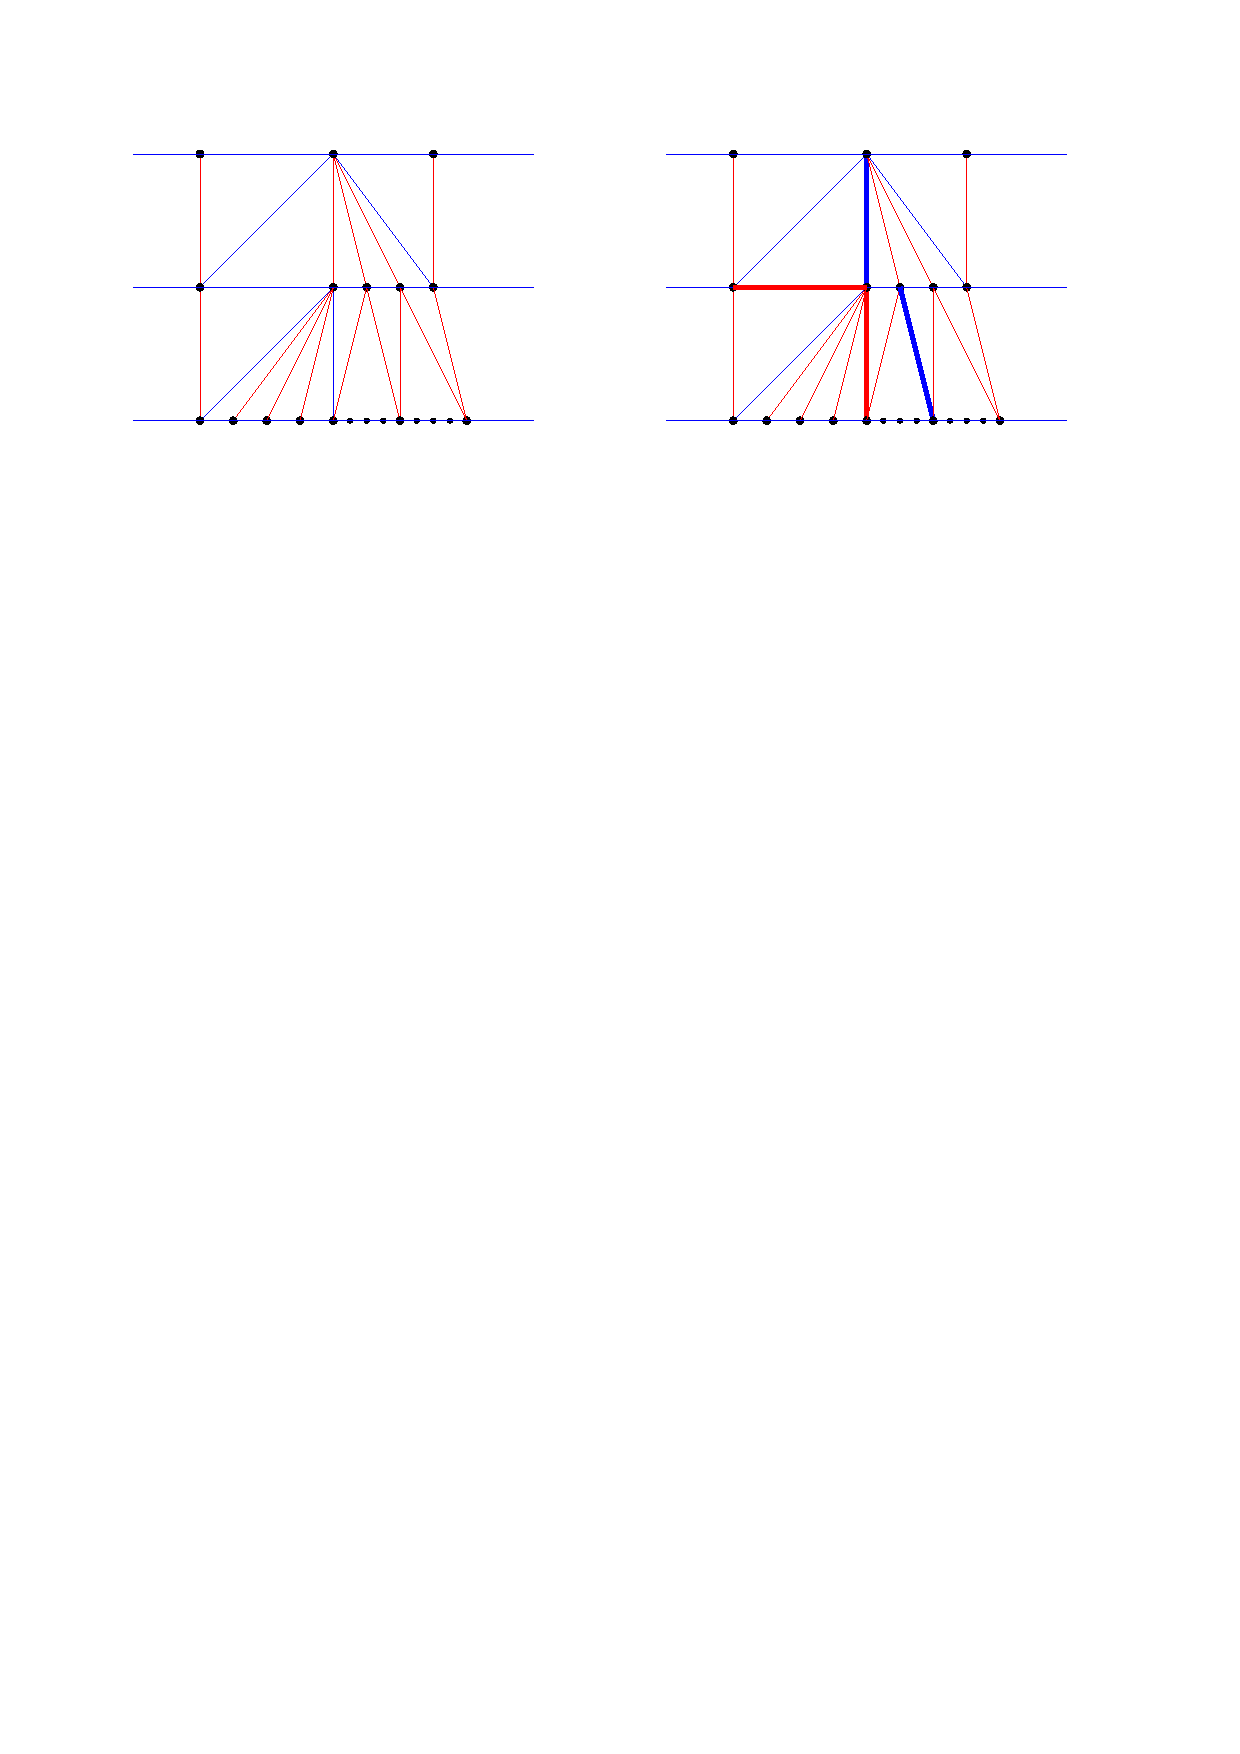
\includegraphics[width =\textwidth]{unifiedAlgo/img/post/sameFlipComplete}
     \caption{The result of both flips}
     \label{fig:uni:sameFlipComplete}
   \end{figure}

   \fxwarning{TODO This flip in a multi case}
   \fxwarning{TODO Argue why these edges are like they are}


   \paragraph{Opposite orientation flips}
   We namely execute the flip given in Figure \ref{fig:uni:oppFlip}. The small vertices on the bottom-left hint on the possibility of vertices but those don't have to be there.

  \begin{figure}[h]
    \centering
    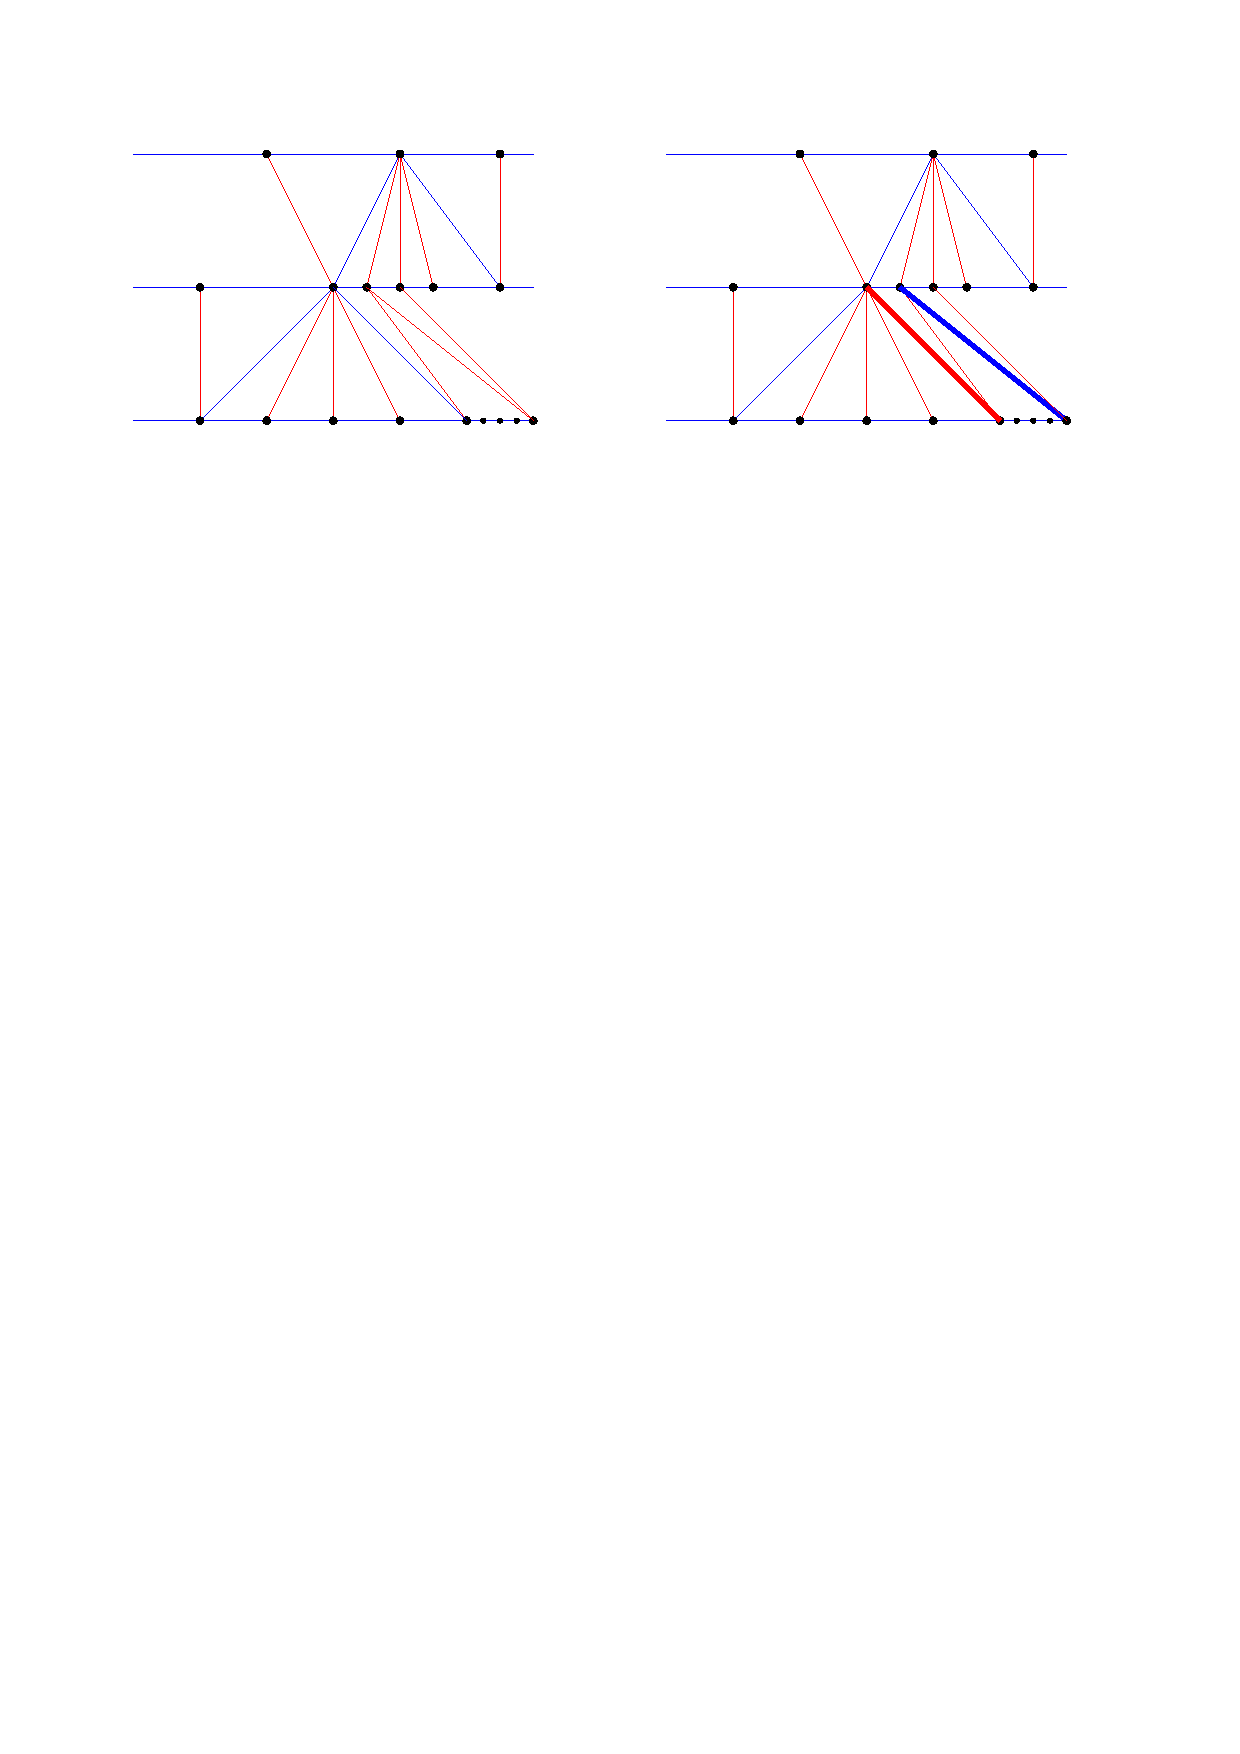
\includegraphics[width = \textwidth]{unifiedAlgo/img/post/oppFlip}
    \caption{The flip we execute on opposite chains}
    \label{fig:uni:oppFlip}
  \end{figure}

  \begin{figure}[h]
    \centering
    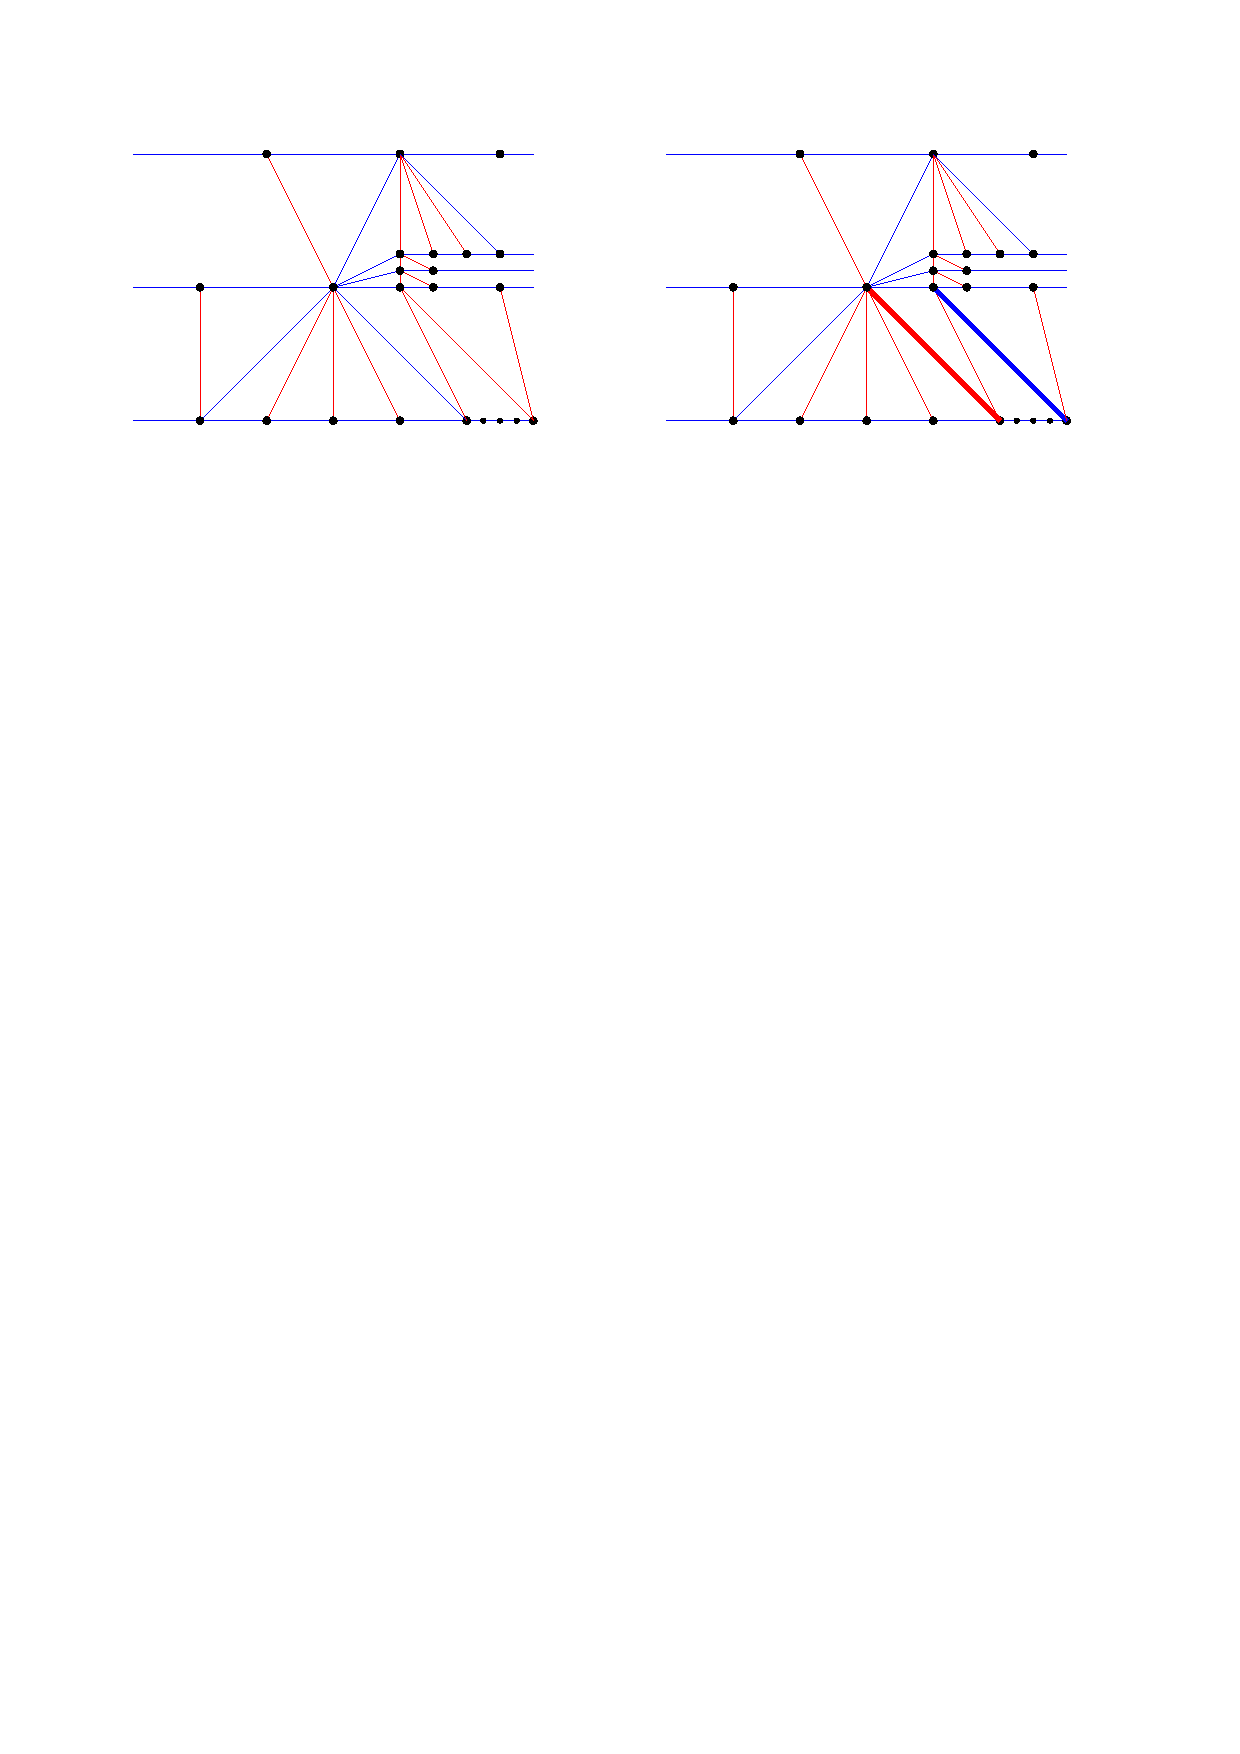
\includegraphics[width = \textwidth]{unifiedAlgo/img/post/oppMultiFlip}
    \caption{The flip we execute on opposite chains with multiple edges in the middle}
    \label{fig:uni:oppMultiFlip}
  \end{figure}

  When recoloring the edge blue in this flip it might be above another $Z$ and thus create a chain of $2$ $Z$'s. However this chain can grow no further as above this newly blue edge there is a red closing triangle.

  \fxwarning{TODO this flip in a multi case}
  \fxwarning{TODO Argue why these edges are like they are}


  \paragraph{Flips with multiple edges in the middle joint.}


  We will want to proof the following about these flips.

  \begin{lemma}
    \label{lm:}
    Faces in already treated strips will never grow with more than $2$ on the top. In particular faces containing a large topfan will remain 3-sided. At the same time there will be no more chains of more then $2$ $Z$'s.
  \end{lemma}

  \begin{proof}
    Let us first describe the effects of both flips.

    We apply a flip when in the current face we discover that we have 2 subsequent $Z$'s. Then applying the flip we change the size of faces in the history. \fxnote{And it will make talking of strips more difficult since we reshape them and not only subdivide them.}

    Let us first describe how these flips change the faces in the historic strips.
    \fxwarning{TODO but first I will describe flips on Z's with a middle fan}
    \begin{figure}[h]
      \centering
      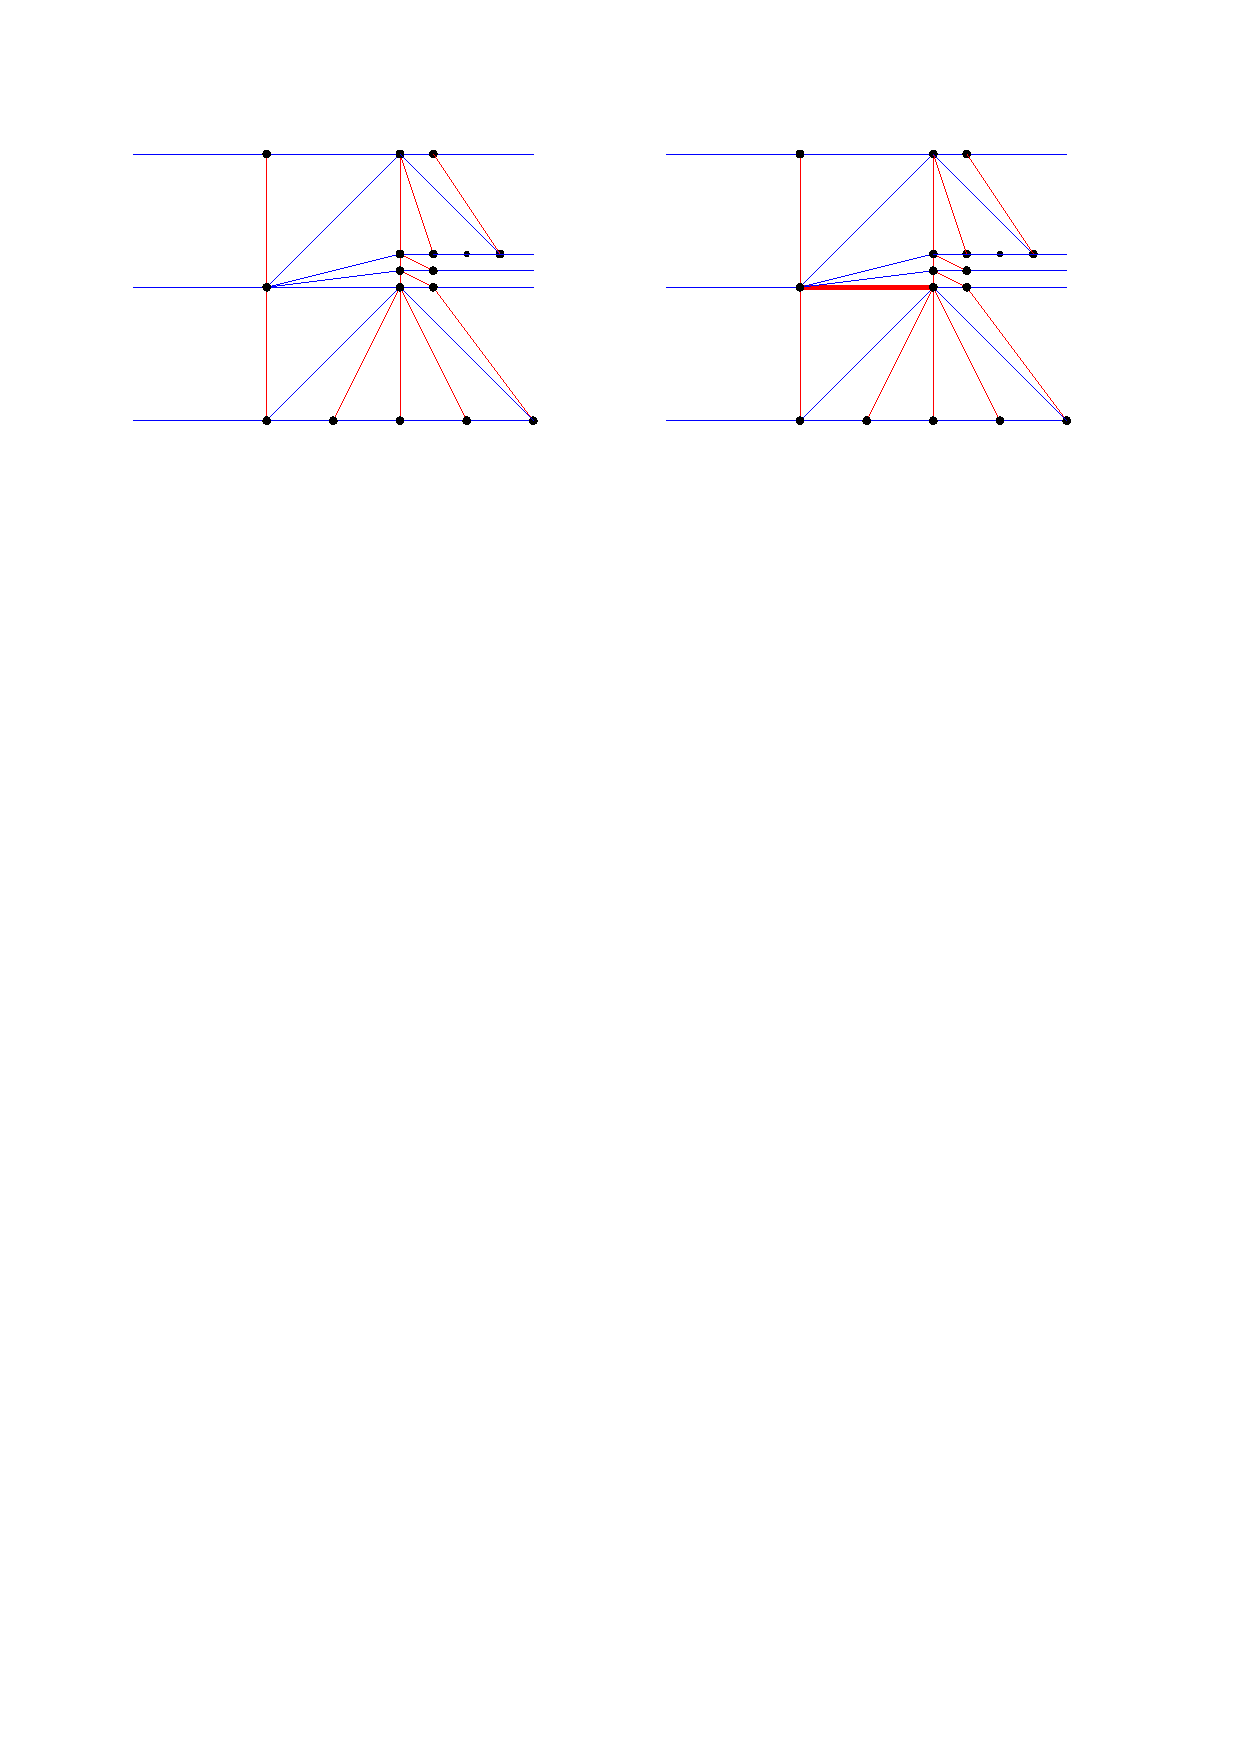
\includegraphics[width =\textwidth]{unifiedAlgo/img/post/sameMultiFlip}
      \caption{The flip we execute on same direction chains with multiple edges in the middle joint}
      \label{fig:uni:sameMultiFlip}
    \end{figure}
    The same orientation flip lengthens one historical face by one vertex on the top and one on the bottom. While the multiflip connects two faces, but will not create a large topfan \fxnote{or maybe one larger. We can definitely connect large topfans this way}.

    The opposite orientation flip follows the same orientation flip without middle edges. And this case it makes one historic face 1-1 longer and another historic face 1-1 shorter. If the shortened face becomes to short we drop this edge.
    The face we elongate now is a different face from the one we elongated in the previous flip.

    Furthermore if we only have to do an opposite chain flip then we simply elongate a face by $1-\infty$ and shorten another face by $1-\infty$. Again we drop the shortened face if it becomes to short (i.e. less then $1-1$)

    \paragraph{Every face is only hit a number of times}
    *Once on each side during same direction flips
    *Once during opp flips (per side)

    OR

    * Just once

    OR

    * We just don't care as long as we don't open topfans (Hint: we don't)
    * However we do enlarge topfans (at most by 1 on every side) so we end up with $3-\infty$ topfans.

    Every two subsequent $Z$'s are treated in one flip. This flip makes a historic faces longer but closes them in such a way they can't be opened by other flips.

    \paragraph{Remaining Z's}
    The opp flip can place an blue edge above another blue edge. However this chain stops here since above this is a red split vertex. So the longest chain of $Z$'s is now of length two.
  \end{proof}
